%%%%%%%%%%%%%%%%%%%%%%%%%%
%%% author : Yamada. T %%%
%%% made for TH series %%%
%%%%%%%%%%%%%%%%%%%%%%%%%%

\documentclass[b5paper,10pt,fleqn] {ltjsarticle}

\usepackage[margin=10truemm]{geometry}

\usepackage{pict2e, graphicx}
\usepackage{tikz}
\usetikzlibrary{intersections,calc,arrows.meta}

\usepackage{amsmath, amssymb, amsthm}
\usepackage{ascmac}
\usepackage{comment}
\usepackage{empheq}
\usepackage[shortlabels,inline]{enumitem}
\usepackage{fancybox}
\usepackage{fancyhdr}
\usepackage{here}
\usepackage{lastpage}
\usepackage{listings, jvlisting}
\usepackage{fixdif}

\usepackage{stmaryrd}
\usepackage[listings]{tcolorbox}
%\usepackage{ascolorbox}
\usepackage{titlesec}
\usepackage{ulem}
\usepackage{url}
\usepackage{verbatim}
\usepackage{wrapfig}
\usepackage{xcolor}
\usepackage{luatexja-ruby}
\usepackage{varwidth}
\usepackage[version=3]{mhchem}
\usepackage{wrapfig}


\usepackage{physics2}
	\usephysicsmodule{ab}
	\usephysicsmodule{ab.braket}
	\usephysicsmodule{ab.legacy}
	%\usephysicsmodule{braket}
	\usephysicsmodule{diagmat}
	\usephysicsmodule{xmat}
	\usephysicsmodule{nabla.legacy}
	\usephysicsmodule{qtext.legacy}

\usepackage[ISO]{diffcoeff}
\difdef { f, s } { D }
{ op-symbol = \mathrm{D} }


\newcommand{\mctext}[1]{\mbox{\textcircled{\scriptsize{#1}}}}
\newcommand{\ctext}[1]{\textcircled{\scriptsize{#1}}}
\newcommand{\ds}{\displaystyle}
\newcommand{\comb}[2]{{}_{#1}\mathrm{C}_{#2}}
\newcommand{\hs}{\hspace}
\newcommand{\vs}{\vspace}
\newcommand{\emphvs}{\vspace{1em}\notag\\}
\newcommand{\ora}{\overrightarrow}
\newcommand{\ol}{\overline}
\newcommand{\oramr}[1]{\overrightarrow{\mathrm{#1}}}
\newcommand{\tri}{\triangle}
\newcommand{\mr}{\mathrm}
\newcommand{\mb}{\mathbb}
\newcommand{\mrvec}[1]{\overrightarrow{\mathrm{#1}}}
\newcommand{\itvec}{\overrightarrow}
\newcommand{\bs}{\boldsymbol}
\newcommand{\ra}{\rightarrow}
\newcommand{\Ra}{\Rightarrow}
\newcommand{\lra}{\longrightarrow}
\newcommand{\Lra}{\Longrightarrow}
\newcommand{\la}{\leftarrow}
\newcommand{\La}{\Leftarrow}
\newcommand{\lla}{\longleftarrow}
\newcommand{\Lla}{\Longleftarrow}
\newcommand{\lr}{\leftrightarrow}
\newcommand{\llr}{\longleftrightarrow}
\newcommand{\Llr}{\Longleftrightarrow}
\renewcommand{\deg}{{}^\circ}
\newcommand{\phbox}{\fbox{\phantom{1\hspace{2em}}}}
\newcommand{\boxnum}[1]{\fbox{\phantom{\hspace{1em}}({#1})\phantom{\hspace{1em}}}}
\newcommand{\boxkana}[1]{\fbox{\phantom{\hspace{1em}}{#1}\phantom{\hspace{1em}}}}
\newcommand{\boxkm}[2]{\fbox{\, {#1}\phantom{\hspace{0.2em}} \,  {#2}}}
\newcommand{\hzw}{\hspace{1\zw}}

\renewcommand{\baselinestretch}{1.25}
\parindent=1\zw

%TH2-7
\begin{document}
\noindent \fbox{NewTH4-3} [東京工業大]

真空中に半径$R$の絶縁体球があり,この球内に単位体積あたり$- \rho\, (\rho > 0)$ の負電荷が一様に分布している.
図1に示すように,この球の中心を含む平面に沿ってせまい隙間を開ける.
平面状の隙間を含む平面を$xy$平面とし,球の中心を座標の原点Oとする.
隙間の幅は無視できるとする.
この隙間内で原点Oより距離$r \, ( \leqq R)$の点における,絶縁体球全体の電荷による電場は,原点Oを中心とする半径$r$の球内に存在する全電荷が原点Oに集中していると考えたときに,この電荷が作る電場と等しいことが知られている.

\begin{figure}[H]
  \centering
  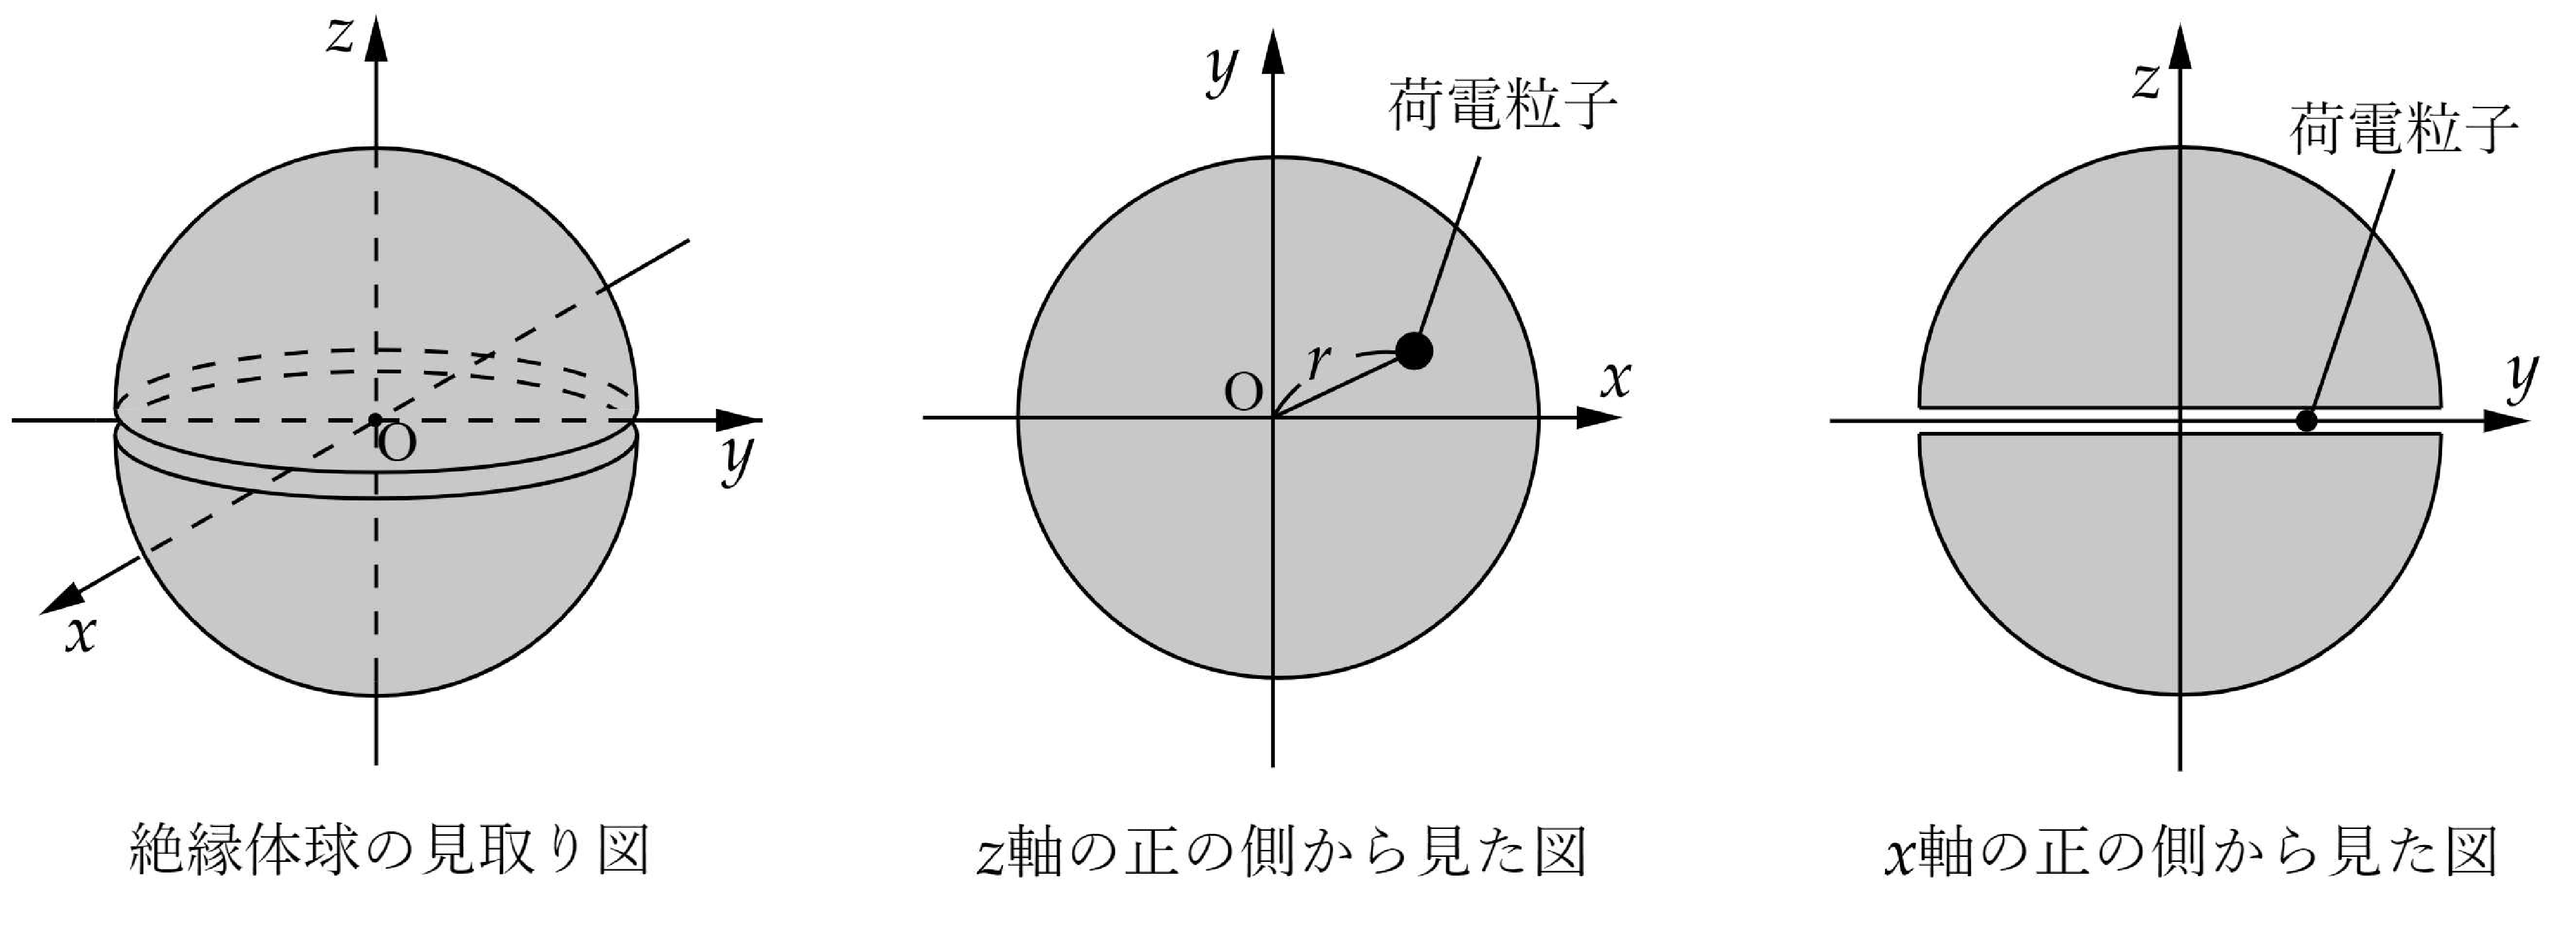
\includegraphics[width=11cm]{fig/fig_4_3_1.pdf}
  \caption{}
\end{figure}

この隙間内で,正電荷$q$を持ち,質量$m$で大きさの無視できる荷電粒子が摩擦なく運動する.以下の問いに答えよ.
ただし,重力の影響を無視し,この荷電粒子は絶縁体球と絶縁されており,この荷電粒子の運動に伴う絶縁体球内の電荷分布の変化はないものとする.

\begin{enumerate}[label = {〔 \Roman* 〕}]
  \item 
    \begin{enumerate}[label={問\arabic*}]
      \setlength{\itemindent}{1\zw}
      \setlength{\labelsep}{1\zw}
      \setlength{\parindent}{1\zw}
      \item 原点Oから距離$r \, ( \leqq R)$にこの荷電粒子があるとき,この荷電粒子の受ける力は原点Oに向かう向きであり,大きさは$F(r) = Cr$と書ける.$C$を求めよ.ただし,真空中のクーロンの法則の比例定数を$k_0$とする.

        以下の問いでは,答に$C$が含まれるときには,問1で得られた$C$の値は代入せずに$C$を用いよ.
      \item $F(r) = Cr$が$r$に比例する形であることに着目して,原点Oから距離$r\, (\leqq R)$にこの荷電粒子があるときの静電気力による位置エネルギー$U(r)$を求めよ.ただし,原点Oを位置エネルギーの基準点にとることにする.
      \item 原点Oにあるこの荷電粒子に$x$軸の正の向きに速さ$v_0$を与える.この荷電粒子が絶縁体球の表面$(r = R)$まで到達するための$v_0$の最小値を求めよ.
    \end{enumerate}
  \item 次に,$z$軸の正の向きに磁束密度の大きさが$B$の一様磁場を加える.
    \begin{enumerate}[label={問\arabic*}, resume]
      \setlength{\itemindent}{1\zw}
      \setlength{\labelsep}{1\zw}
      \setlength{\parindent}{1\zw}

      \item 問3と同様に,原点Oにあるこの荷電粒子に$x$軸の正の向きに速さ$v_1$を与えたところ.図2に示す曲線に沿ってこの荷電粒子は運動し,絶縁体球の表面に到達した.球の表面に到達したときのこの荷電粒子の速さ$v$を求めよ.
      \begin{figure}[H]
        \centering
        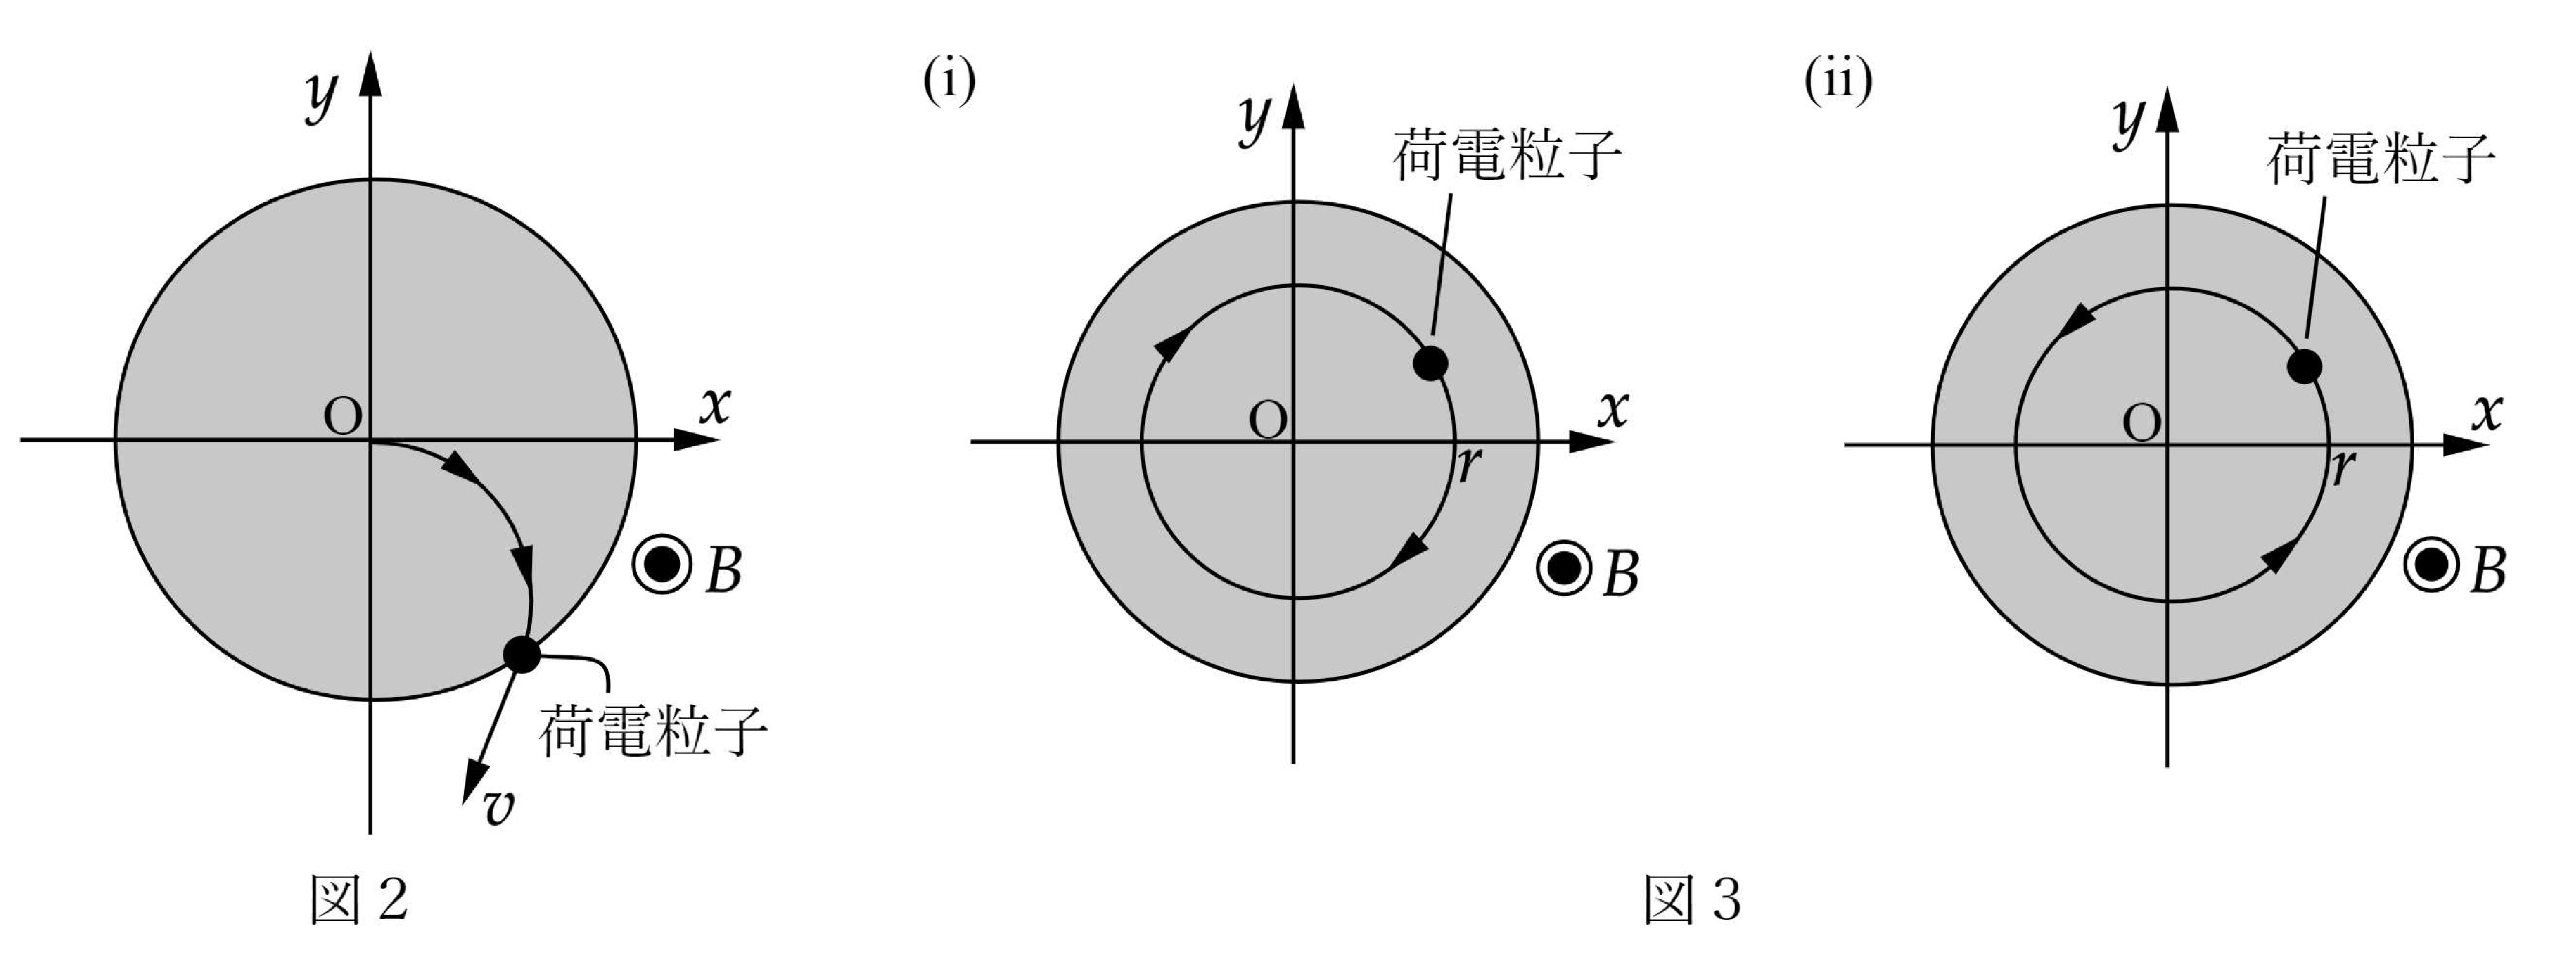
\includegraphics[width=11cm]{fig/fig_4_3_2.pdf}
      \end{figure}
      \item 原点Oから距離$r \, (< R)$にあるこの荷電粒子に適当な速度を与えると,この荷電粒子が隙間内で原点Oを中心とする半径$r$の等速円運動を行う.図3に示すように,円運動が$xy$平面内で(i)時計回りのとき,(ii)反時計回りのとき,それぞれについて円運動の角速度の大きさを求めよ. 
      \item  以下の空欄に入る適切な数式を答えよ.

        問5では,この荷電粒子の円運動が(i)時計回りのときと(ii)反時計回りのときとで角速度の大きさが異なっている.もし,この荷電粒子の運動を,原点Oを中心として,角速度$\Omega = \text{\boxnum{1}}$で$xy$面内を時計回りに回転運動している観測者Kから見ると,(i)時計回りのときと(ii)反時計回りのときとでこの荷電粒子の円運動の角速度の大きさは等しく,ともに$\omega ' = \text{\boxnum{2}}$と観測される.

        これは物理的には次のように解釈できる.観測者Kから見たときの電場や磁場の観測値は,静止している観測者Sから見たときとは異なる.観測者Kから観測すると,この隙間内の磁場はなく,電場は原点Oに向かう向きとなっている.このために,観測者Kから見たときのこの荷電粒子の円運動の角速度の大きさが,(i)時計回りのときと(ii)反時計回りのときとで等しくなっている.また,観測者Kから見たときの電場からこの荷電粒子が受ける力の大きさは$F(r) = C' r$($C'$は定数)と書ける.ここで,$C' = \text{\boxnum{3}}$であり,この値は$C$とは異なっていて,確かに電場の観測値は,観測者Kと観測者Sとで異なっていることがわかる.
    \end{enumerate}
\end{enumerate}
\end{document}
